\header{
    \headtitle{Je l'aide à vomir} \label{je-l-aide-a-vomir}
    %
    
    \insertComment{Sur l'air de "Je l'aime à mourir" de F. Cabrel (1979).}{}
}

\enluminure{4}{\href{https://www.youtube.com/watch?v=bMZVtFCU0ZQ}{M}}{oi} je n'étais rien et voilà qu'aujourd'hui
\\Je suis le gardien de l'ivresse de ses nuits
\\Je l'aide à vomir
\\Vous pouvez couvrir tout ce qui vous plaira
\\Elle n'aura qu'à ouvrir l'antre et le cardia
\\Pour tout vous pourrir \bissimple
\\Je l'aide à vomir.
\\\\\textbf{Refrain :}
\\Elle a du boire toutes les bières
\\Pour être aussi morte aujourd'hui,
\\Elle a du boire bien trop de bières
\\Du Ricard aussi.
\\\\Elle boit de son mieux des litres de Gin
\\Elle danse au milieu des bouteilles qu'elle chopine
\\Je l'aide à vomir
\\Elle a tombé les dents à force de picoler
\\Elle me chante souvent qu'elle essaye d'arrêter
\\Pour me retenir \bissimple
\\Je l'aide à vomir.
\\\\Elle produit sa gnole cachée sous les toits
\\Je dois finir ses groles qui me mettent à plat
\\Je l'aide à vomir
\\Je la couche le soir, et pour bien dégueuler
\\Elle dort dans la baignoire et finit par gerber
\\Sans rien retenir \bissimple
\\Je l'aide à vomir.
\breakpage
Moi je n'étais rien et voilà qu'aujourd'hui
\\Je suis le gardien de l'ivresse de ses nuits
\\Je l'aide à vomir
\\Vous pouvez couvrir tout ce qui vous plaira
\\Elle n'aura qu'à ouvrir l'antre et le cardia
\\Pour tout vous pourrir \bissimple
\\Je l'aide à vomir.
\\
\begin{figure}[h!]
\centering
   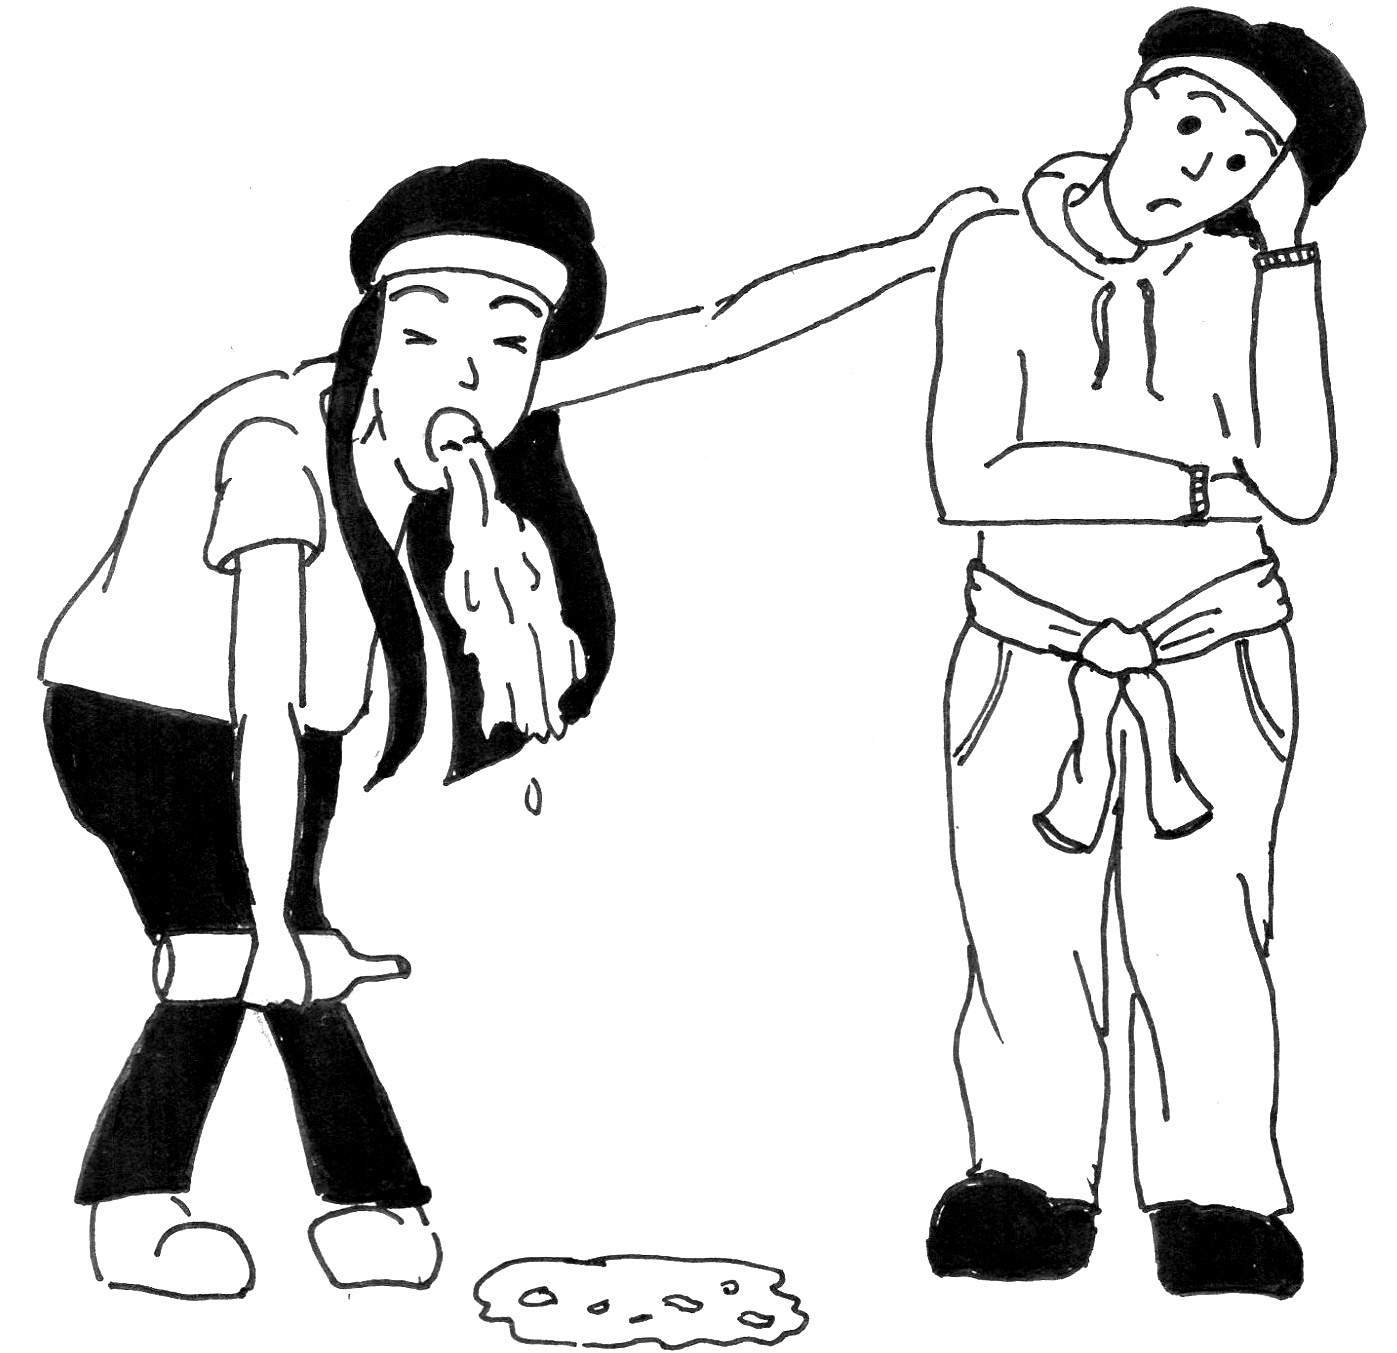
\includegraphics[width=1\textwidth]{images/aide_a_vomir.jpg}
 \end{figure}

\breakpage